\documentclass[12pt]{article}
\usepackage[utf8]{inputenc}
\usepackage[T1]{fontenc}
\usepackage[spanish]{babel}%caracteres en español
\usepackage{verbatim}
\title{\huge \textbf{\textsc{Actividad 6 \\ Análisis armónico de mareas}}}%titulo en grande-negritas-versalitas
\author{Jesús Ernesto Torres Burruel}
\usepackage{graphicx}%para cargar imagenes
\graphicspath{{Imagenes/}}
\usepackage{wrapfig} %para acomodar figuras y que compartan espacio con texto
\usepackage{fancyhdr}
\pagestyle{fancy}
\fancyhf{}
\usepackage{enumerate}
\usepackage{cite}
\usepackage{hyperref}
\usepackage{bookmark}
\fancyfoot[R]{Página \thepage}
\setlength\headheight{15 pt}
\fancyhead[L]{J. Ernesto Torres Burruel}
\fancyhead[R]{Física Computacional I}
\usepackage{booktabs}
\usepackage[nottoc,numbib]{tocbibind}

\date{15 de mayo del 2017}
\begin{document}

\begin{titlepage}

    \begin{figure}[ht!]
    \centering
    \includegraphics[scale = 0.25]{logo}
    
    \textbf{UNIVERSIDAD DE SONORA \\ DIVISIÓN DE CIENCIAS EXACTAS Y NATURALES \\ DEPARTAMENTO DE FÍSICA \\ LICENCIATURA EN FÍSICA}
	\maketitle
    \hrule \bigskip
    \large{Física Computacional I}\\
	Profr. Carlos Lizárraga Celaya
    \end{figure}
\thispagestyle{empty}

\end{titlepage}

\newpage

\begin{center}
\huge{\textbf{\textsc{El sistema de Lorenz}}}
\end{center}
\noindent Edward Norton Lorenz (23 de mayo de 1917 - 16 de Abril de 2008) fue un matemático y meteorólogo estadounidense, además de ser un pionero de la teoría del caos; fue Lorenz quien introdujo el término de atractor extraño y acuñó el término de efecto mariposa.\cite{lorenz}

En sus trabajos sobre atmósfera, al tratar de reducir y simplificar las ecuaciones para describir el estado de la atmósfera llegó a un modelo que parecía bastante simple, sin embargo llevó a toda una nueva teoría, tal vez no para la atmósfera pero sí para las matemáticas y la percepción de los problemas que se ven afectados por el más mínimo cambio.

\section{Sistema de Lorenz}
\noindent El sistema de Lorenz es un sistema de ecuaciones diferenciales ordinarias, estudiadas por primera vez por Edward Lorenz. Este sistema se caracteriza por tener soluciones caóticas bajo ciertas condiciones iniciales, especialmente el atractor de Lorenz es un conjunto de soluciones caóticas que al ser graficadas se asemejan a una mariposa, es por eso que a se tiene el nombre del efecto mariposa para las situaciones en las que el más mínimo cambio afecta a todo el sistema.\cite{video}

\subsection{Simplificación del modelo atmosférico}
\noindent En 1963 Lorenz trabajó en la simplificación del modelo matemático para la convección atmosférica, llegó a un sistema tan simplificado que podría ya no tener ninguna relación con el análisis atmosférico. Debido al modelo tan simple al que llegó se le denominó modelo de juguete, pues el modelo del comportamiento de la atmósfera llegó a depender de solo tres parámetros.

LAs ecuaciones diferenciales que representan al sistema de Lorenz son:
\begin{align*}
\frac{\delta x}{\delta t} &= \sigma \left( y- x \right), \\
\frac{\delta y}{\delta t} &= x \left( \rho- z \right) -y, \\
\frac{\delta z}{\delta t} &= xy - \beta z,
\end{align*}
donde $x$, $y$, $z$ representan el estado del sistema, $t$ es el tiempo y $\sigma$, $\rho$ y $\beta$ son los parámetros del sistema. Las ecuaciones de Lorenz surgen también al simplificar otros modelos y ha sido  objeto de una gran cantidad de articulos de investigación, eso sin mencionar que impulsó la teoría del caos.

\section{Análisis del sistema}
Si se consideran a los parámetros como
\begin{align*}
\sigma & = 10 \\
\beta & = \frac{8}{3} \\
\rho & = 28
\end{align*}
El sistema presenta un comportamiento caótico, casi todos los puntos tienden al atractor de Lorenz y a un fractal, el atractor de Lorenz es denominado un atractor extraño, pues es el nombre que recibe por el comportamiento que presentan las trayectorias que son solución al sistema.\cite{atractor}

En las figuras \ref{lg}, \ref{lxy}, \ref{lxz}, \ref{lyz} y \ref{ld} se tiene la visualización de la solución al sistema de Lorenz bajo estos parámetros.\footnote{Los gráficos fueron generados a partir del código proporcionado como ejemplo por matplotlib \\ \url{https://matplotlib.org/2.0.0/examples/mplot3d/lorenz_attractor.html}}

\begin{figure}[p!]
\centering
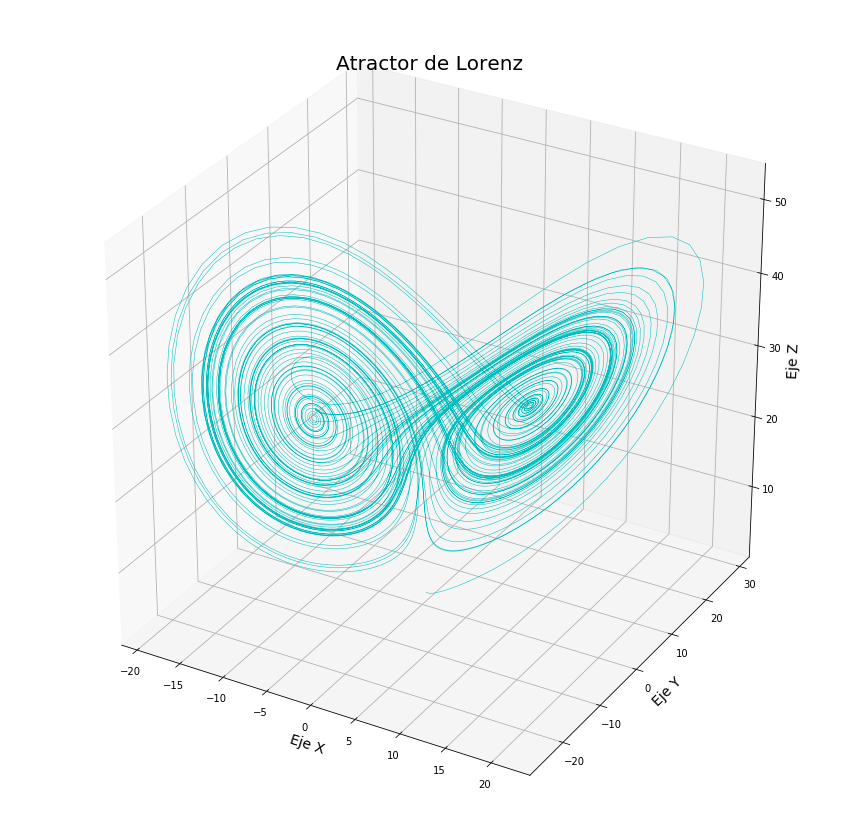
\includegraphics[width= 0.9 \textwidth]{ltzg}
\caption{Proyección en 3D de la solución al sistema de Lorenz con parámetros $\sigma = 10$, $\beta = \frac{8}{3}$, $\rho = 28$}
\label{lg}
\end{figure}

\begin{figure}[p!]
\centering
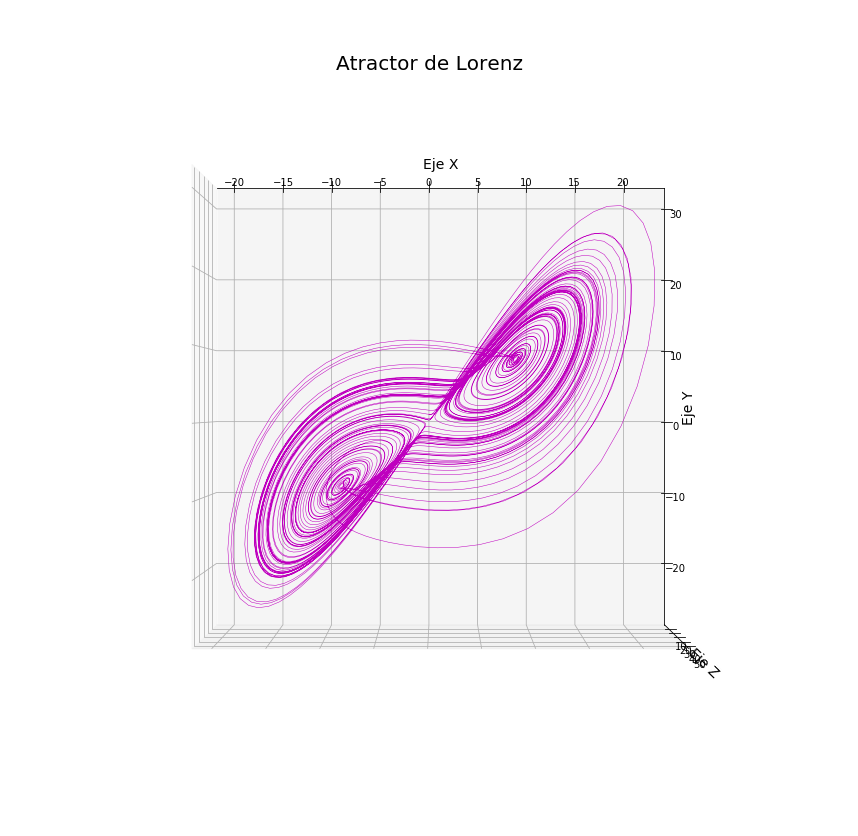
\includegraphics[width= 0.9 \textwidth]{ltzxy}
\caption{Proyección vista sobre el plano xy de la solución al sistema de Lorenz con parámetros $\sigma = 10$, $\beta  = \frac{8}{3}$, $\rho = 28$}
\label{lxy}
\end{figure}

\begin{figure}[p!]
\centering
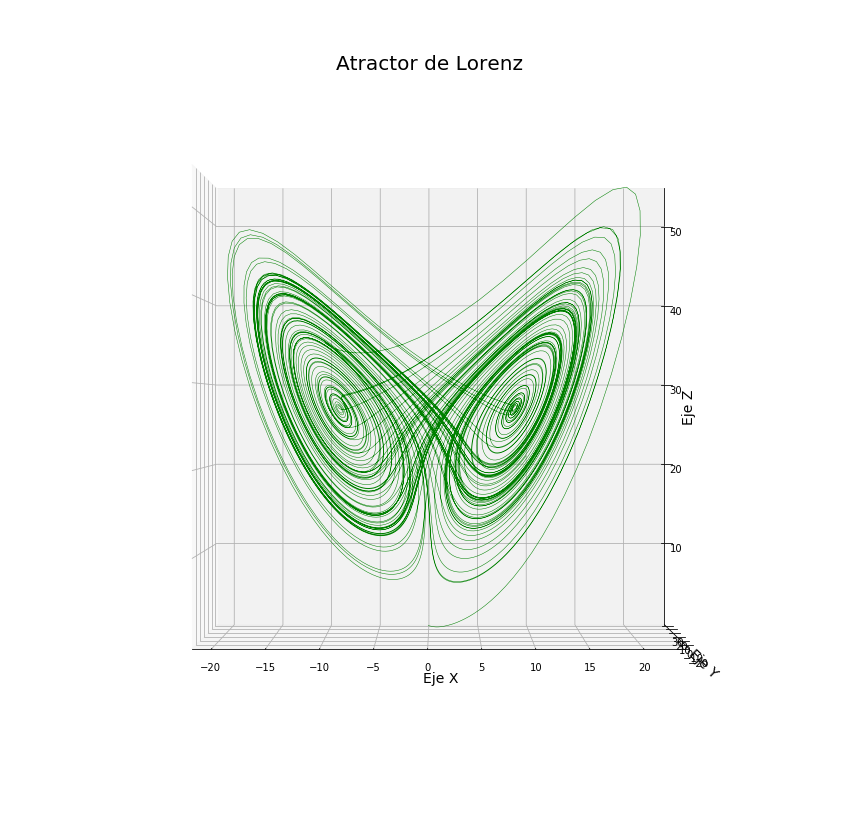
\includegraphics[width= 0.9 \textwidth]{ltzxz}
\caption{Proyección vista sobre el plano xz de la solución al sistema de Lorenz con parámetros $\sigma  = 10$, $\beta  = \frac{8}{3}$, $\rho = 28$}
\label{lxz}
\end{figure}

\begin{figure}[p!]
\centering
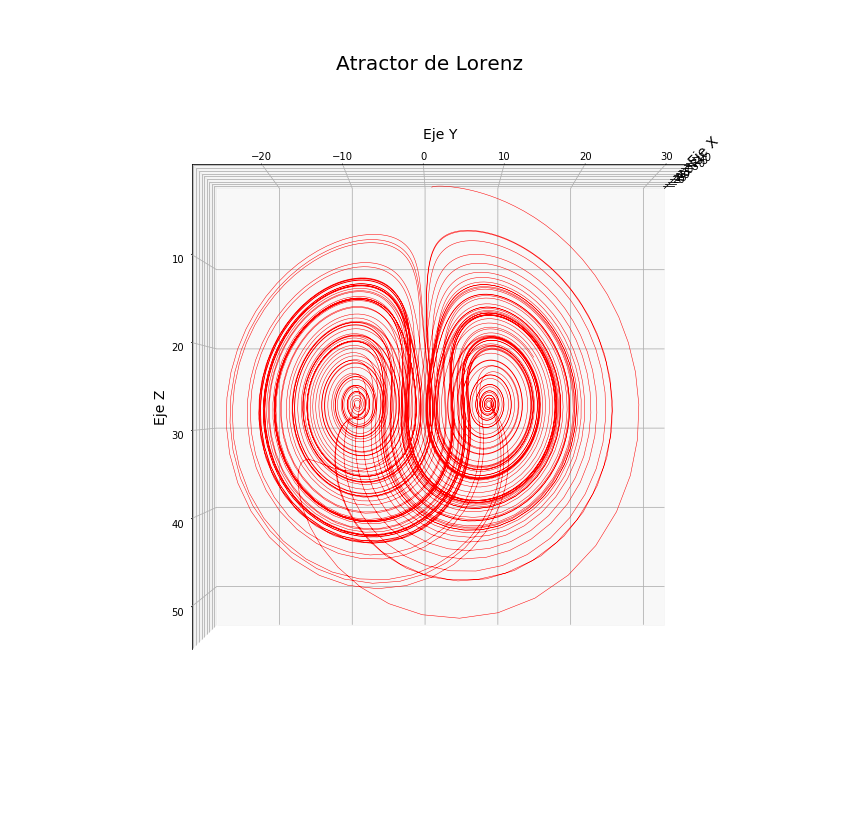
\includegraphics[width= 0.9 \textwidth]{ltzyz}
\caption{Proyección vista sobre el plano yz de la solución al sistema de Lorenz con parámetros $\sigma  = 10$, $\beta  = \frac{8}{3}$, $\rho  = 28$}
\label{lyz}
\end{figure}

\begin{figure}[p!]
\centering
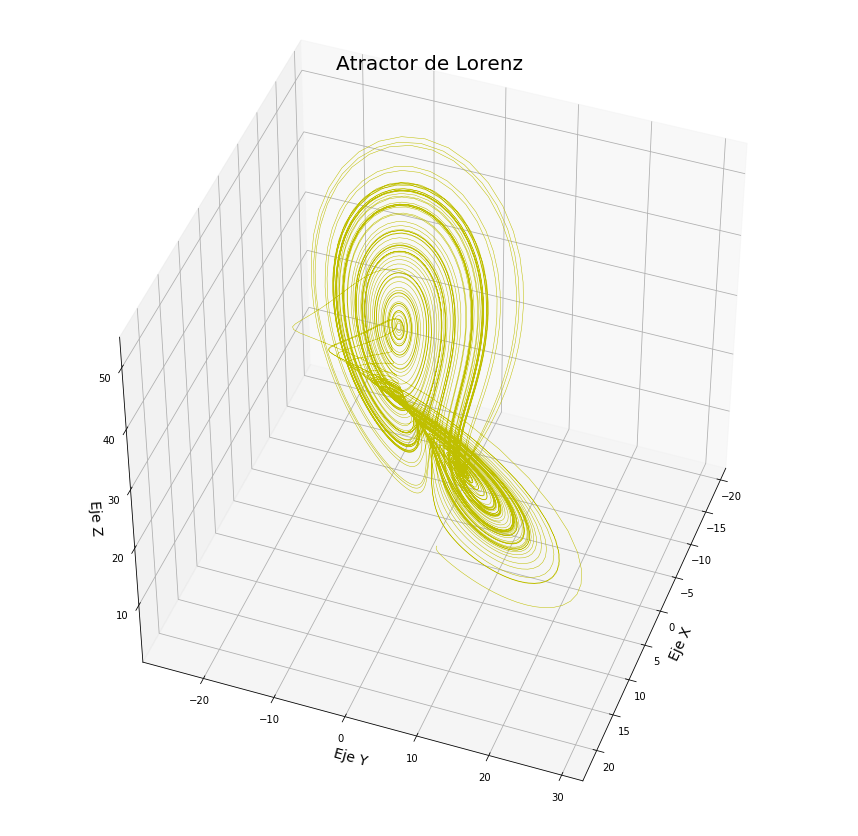
\includegraphics[width= 0.9 \textwidth]{ltzd}
\caption{Proyección en 3D rotada de la solución al sistema de Lorenz con parámetros $\sigma  = 10$, $\beta  = \frac{8}{3}$, $\rho = 28$}
\label{ld}
\end{figure}

\pagebreak

\newpage

\section*{Apéndice A: código utilizado para las visualizaciones del sistema de Lorenz}
\begin{verbatim}
import numpy as np
import matplotlib.pyplot as plt
from mpl_toolkits.mplot3d import Axes3D


def lorenz(x, y, z, s=10, r=28, b=2.667):
    x_dot = s*(y - x)
    y_dot = r*x - y - x*z
    z_dot = x*y - b*z
    return x_dot, y_dot, z_dot

dt = 0.01
stepCnt = 10000

# Se necesita uno más para los valores iniciales
xs = np.empty((stepCnt + 1,))
ys = np.empty((stepCnt + 1,))
zs = np.empty((stepCnt + 1,))

# Valores iniciales
xs[0], ys[0], zs[0] = (0., 1., 1.05)

# Posicionamiento con respecto al tiempo.
for i in range(stepCnt):
    # Derivatives of the X, Y, Z state
    x_dot, y_dot, z_dot = lorenz(xs[i], ys[i], zs[i])
    xs[i + 1] = xs[i] + (x_dot * dt)
    ys[i + 1] = ys[i] + (y_dot * dt)
    zs[i + 1] = zs[i] + (z_dot * dt)

fig = plt.figure(figsize=(15,15))
ax = fig.gca(projection='3d')

ax.plot(xs, ys, zs, color='nombre del color' , lw=0.5)
ax.set_xlabel('Eje X', fontsize= 14)
ax.set_ylabel("Eje Y", fontsize= 14)
ax.set_zlabel("Eje Z", fontsize= 14)
ax.set_title("Atractor de Lorenz", fontsize= 20)

ax.view_init(grados de altitud, grados de azimutal)
plt.show()
\end{verbatim}
\pagebreak
\newpage

\section*{Apéndice B: Código para realizar animaciones}
Los siguientes códigos son utilizados para realizar animaciones del sistema de Lorenz y permiten la visualización del comportamiento del sistema al transcurrir el tiempo y con visualizaciones a distintos ángulos. Los códigos fueron proporcionados por Goeff Boeing y el usuario de Disqus \textit{jakevdp}. (Los productos de estos códigos pueden verse en \url{https://github.com/ErnestoTb/Computacional1/tree/master/Actividad\%208/Imagenes\%20y\%20animaciones}

\begin{verbatim}

# coding: utf-8

# ## El atractor de Lorenz


get_ipython().magic('matplotlib inline')
import numpy as np, matplotlib.pyplot as plt, glob, os
import IPython.display as IPdisplay, matplotlib.font_manager as fm
from scipy.integrate import odeint
from mpl_toolkits.mplot3d.axes3d import Axes3D
from PIL import Image


# define the fonts to use for plots
family = 'Myriad Pro'
title_font = fm.FontProperties(family=family, style='normal', size=20, 
weight='normal', stretch='normal')



save_folder = 'images/lorenz-animate'
if not os.path.exists(save_folder):
    os.makedirs(save_folder)



# define the initial system state (aka x, y, z positions in space)
initial_state = [0.1, 0, 0]

# define the system parameters sigma, rho, and beta
sigma = 10.
rho   = 28.
beta  = 8./3.

# define the time points to solve for, evenly spaced between the start 
and end times
start_time = 1
end_time = 60
interval = 100
time_points = np.linspace(start_time, end_time, end_time * interval)



# define the lorenz system
def lorenz_system(current_state, t):
    x, y, z = current_state
    dx_dt = sigma * (y - x)
    dy_dt = x * (rho - z) - y
    dz_dt = x * y - beta * z
    return [dx_dt, dy_dt, dz_dt]



# plot the system in 3 dimensions
from matplotlib import cm
def plot_lorenz(xyz, n):
    fig = plt.figure(figsize=(12, 9))
    ax = fig.gca(projection='3d')
    ax.xaxis.set_pane_color((1,1,1,1))
    ax.yaxis.set_pane_color((1,1,1,1))
    ax.zaxis.set_pane_color((1,1,1,1))
    x = xyz[:, 0]
    y = xyz[:, 1]
    z = xyz[:, 2]
    
    ax.plot(x, y, z, color= "turquoise", alpha=0.7, linewidth=0.7)
    ax.set_xlim((-30,30))
    ax.set_ylim((-30,30))
    ax.set_zlim((0,50))
    ax.set_title('Lorenz system attractor', fontproperties=title_font)
    
    plt.savefig('{}/{:03d}.png'.format(save_folder, n), dpi=60, 
    bbox_inches='tight', pad_inches=0.1)
    plt.close()



# return a list in iteratively larger chunks
def get_chunks(full_list, size):
    size = max(1, size)
    chunks = [full_list[0:i] for i in range(1, len(full_list) + 1, 
    size)]
    return chunks



# get incrementally larger chunks of the time points, to reveal the 
attractor one frame at a time
chunks = get_chunks(time_points, size=20)



# get the points to plot, one chunk of time steps at a time, by 
integrating the system of equations
points = [odeint(lorenz_system, initial_state, chunk) for chunk in 
chunks]



# plot each set of points, one at a time, saving each plot
for n, point in enumerate(points):
    plot_lorenz(point, n)


# # Animación


# create a tuple of display durations, one for each frame
first_last = 100 #show the first and last frames for 100 ms
standard_duration = 5 #show all other frames for 5 ms
durations = tuple([first_last] + [standard_duration] * (len(points) - 
2) + [first_last])



# load all the static images into a list
images = [Image.open(image) for image in 
glob.glob('{}/*.png'.format(save_folder))]
gif_filepath = 'images/animated-lorenz-attractor.gif'



# save as an animated gif
gif = images[0]
gif.info['duration'] = durations #ms per frame
gif.info['loop'] = 0 #how many times to loop (0=infinite)
gif.save(fp=gif_filepath, format='gif', save_all=True, 
append_images=images[1:])



# verify that the number of frames in the gif equals the number of 
image files and durations
Image.open(gif_filepath).n_frames == len(images) == len(durations)


IPdisplay.Image(url=gif_filepath)


# ## Código de animación alternativo
# - https://jakevdp.github.io/blog/2013/02/16/animating-the-lorentz-
system-in-3d/

import numpy as np
from scipy import integrate

# Note: t0 is required for the odeint function, though it's not used 
here.
def lorentz_deriv(params, t0, sigma=10., beta=8./3, rho=28.0):
    """Compute the time-derivative of a Lorentz system."""
    x, y, z = params
    return [sigma * (y - x), x * (rho - z) - y, x * y - beta * z]

x0 = [1, 1, 1]  # starting vector
t = np.linspace(0, 3, 1000)  # one thousand time steps
x_t = integrate.odeint(lorentz_deriv, x0, t)


import numpy as np
from scipy import integrate

from matplotlib import pyplot as plt
from mpl_toolkits.mplot3d import Axes3D
from matplotlib.colors import cnames
from matplotlib import animation

N_trajectories = 20


def lorentz_deriv(params, t0, sigma=10., beta=8./3, rho=28.0):
    """Compute the time-derivative of a Lorentz system."""
    x, y, z = params
    return [sigma * (y - x), x * (rho - z) - y, x * y - beta * z]


# Elige valores iniciales aleatorios uniformemente distribuidos de -15 a 15
np.random.seed(1)
x0 = -15 + 30 * np.random.random((N_trajectories, 3))

# Solve for the trajectories
t = np.linspace(0, 4, 1000)
x_t = np.asarray([integrate.odeint(lorentz_deriv, x0i, t)
                  for x0i in x0])

# Establecer figura y ejes 3D para animación
fig = plt.figure(figsize=(10,10))
ax = fig.add_axes([0, 0, 1, 1], projection='3d')
ax.axis('off')

# Colores diferentes para cada trayectoria
colors = plt.cm.cool(np.linspace(0, 1, N_trajectories))

# Establecer lineas y puntos
lines = [ax.plot([], [], [], '-', c=c)[0]
for c in colors]
pts = [ax.plot([], [], [], 'o', c=c)[0]
for c in colors]

# Límites de los ejes
ax.set_xlim((-25, 25))
ax.set_ylim((-35, 35))
ax.set_zlim((5, 55))

# Punto de vista del objeto (grados de altitud, grados de azimutal)
ax.view_init(30, 0)

# Inicialización de la función: grafica el fondo para cada marco
def init():
    for line, pt in zip(lines, pts):
        line.set_data([], [])
        line.set_3d_properties([])

        pt.set_data([], [])
        pt.set_3d_properties([])
    return lines + pts

# Funcion de animacion. Esto va a ser llamado secuencialmente con el 
número de figura
def animate(i):
# Avanzará dos pasos de tiempo por figura para tener mejores resultados.
    i = (2 * i) % x_t.shape[1]

    for line, pt, xi in zip(lines, pts, x_t):
        x, y, z = xi[:i].T
        line.set_data(x, y)
        line.set_3d_properties(z)

        pt.set_data(x[-1:], y[-1:])
        pt.set_3d_properties(z[-1:])

    ax.view_init(30, 0.3 * i)
    fig.canvas.draw()
    return lines + pts

# Inctancia del animador
anim = animation.FuncAnimation(fig, animate, init_func=init,
                               frames=500, interval=30, blit=True)

#Guardar como .mp4 (Requiere mplayer o ffmpeg instalados)
anim.save('lorentz_attractorg1.mp4', fps=15, extra_args=['-vcodec', 'libx264'])

plt.show()
\end{verbatim}
\pagebreak

\newpage

\nocite{caos}
\bibliographystyle{IEEEtran}
\bibliography{referencias}
\end{document}